\subsection{Real data}
\label{subsection:real_data}
    \noindent
    Mexico city is considered one of the densely populated urban areas with a population that surpasses $20$ million. Consequently, Mexico city faces significant challenges related to water management frequently encountering situations where water demand exceeds the available supply.  To address this issue, the city relies on groundwater extraction leading to occurrences of subsidence and deformations in the land. We investigate a pile of $20$ Sentinel-$1$ \acs{SAR} images covering Mexico city, acquired every $12$ days from August $14$, $2019$, to April $10$, $2020$ to evaluate the effectiveness of the proposed approach.
    %\begin{figure*}[t] % Utilisation de l'environnement figure* pour prendre toute la largeur
    %\centering
    %\begin{minipage}{0.24\textwidth}
    %    \includegraphics[width=\linewidth]{image1.jpg}
    %    \caption*{Image 1} % Légende sans numéro
    %\end{minipage}%
    %\hfill
    %\begin{minipage}{0.24\textwidth}
    %    \includegraphics[width=\linewidth]{image2.jpg}
    %    \caption*{Image 2}
    %\end{minipage}%
    %\hfill
    %\begin{minipage}{0.24\textwidth}
    %    \includegraphics[width=\linewidth]{image3.jpg}
    %    \caption*{Image 3}
    %\end{minipage}%
    %\hfill
    %\begin{minipage}{0.24\textwidth}
    %    \includegraphics[width=\linewidth]{image4.jpg}
    %    \caption*{Image 4}
    %\end{minipage}
    %\end{figure*}
    \vspace{-0.5cm}
    \begin{figure}[!h]
        \centering
        \begin{subfigure}[b]{\columnwidth}
            \centering
            %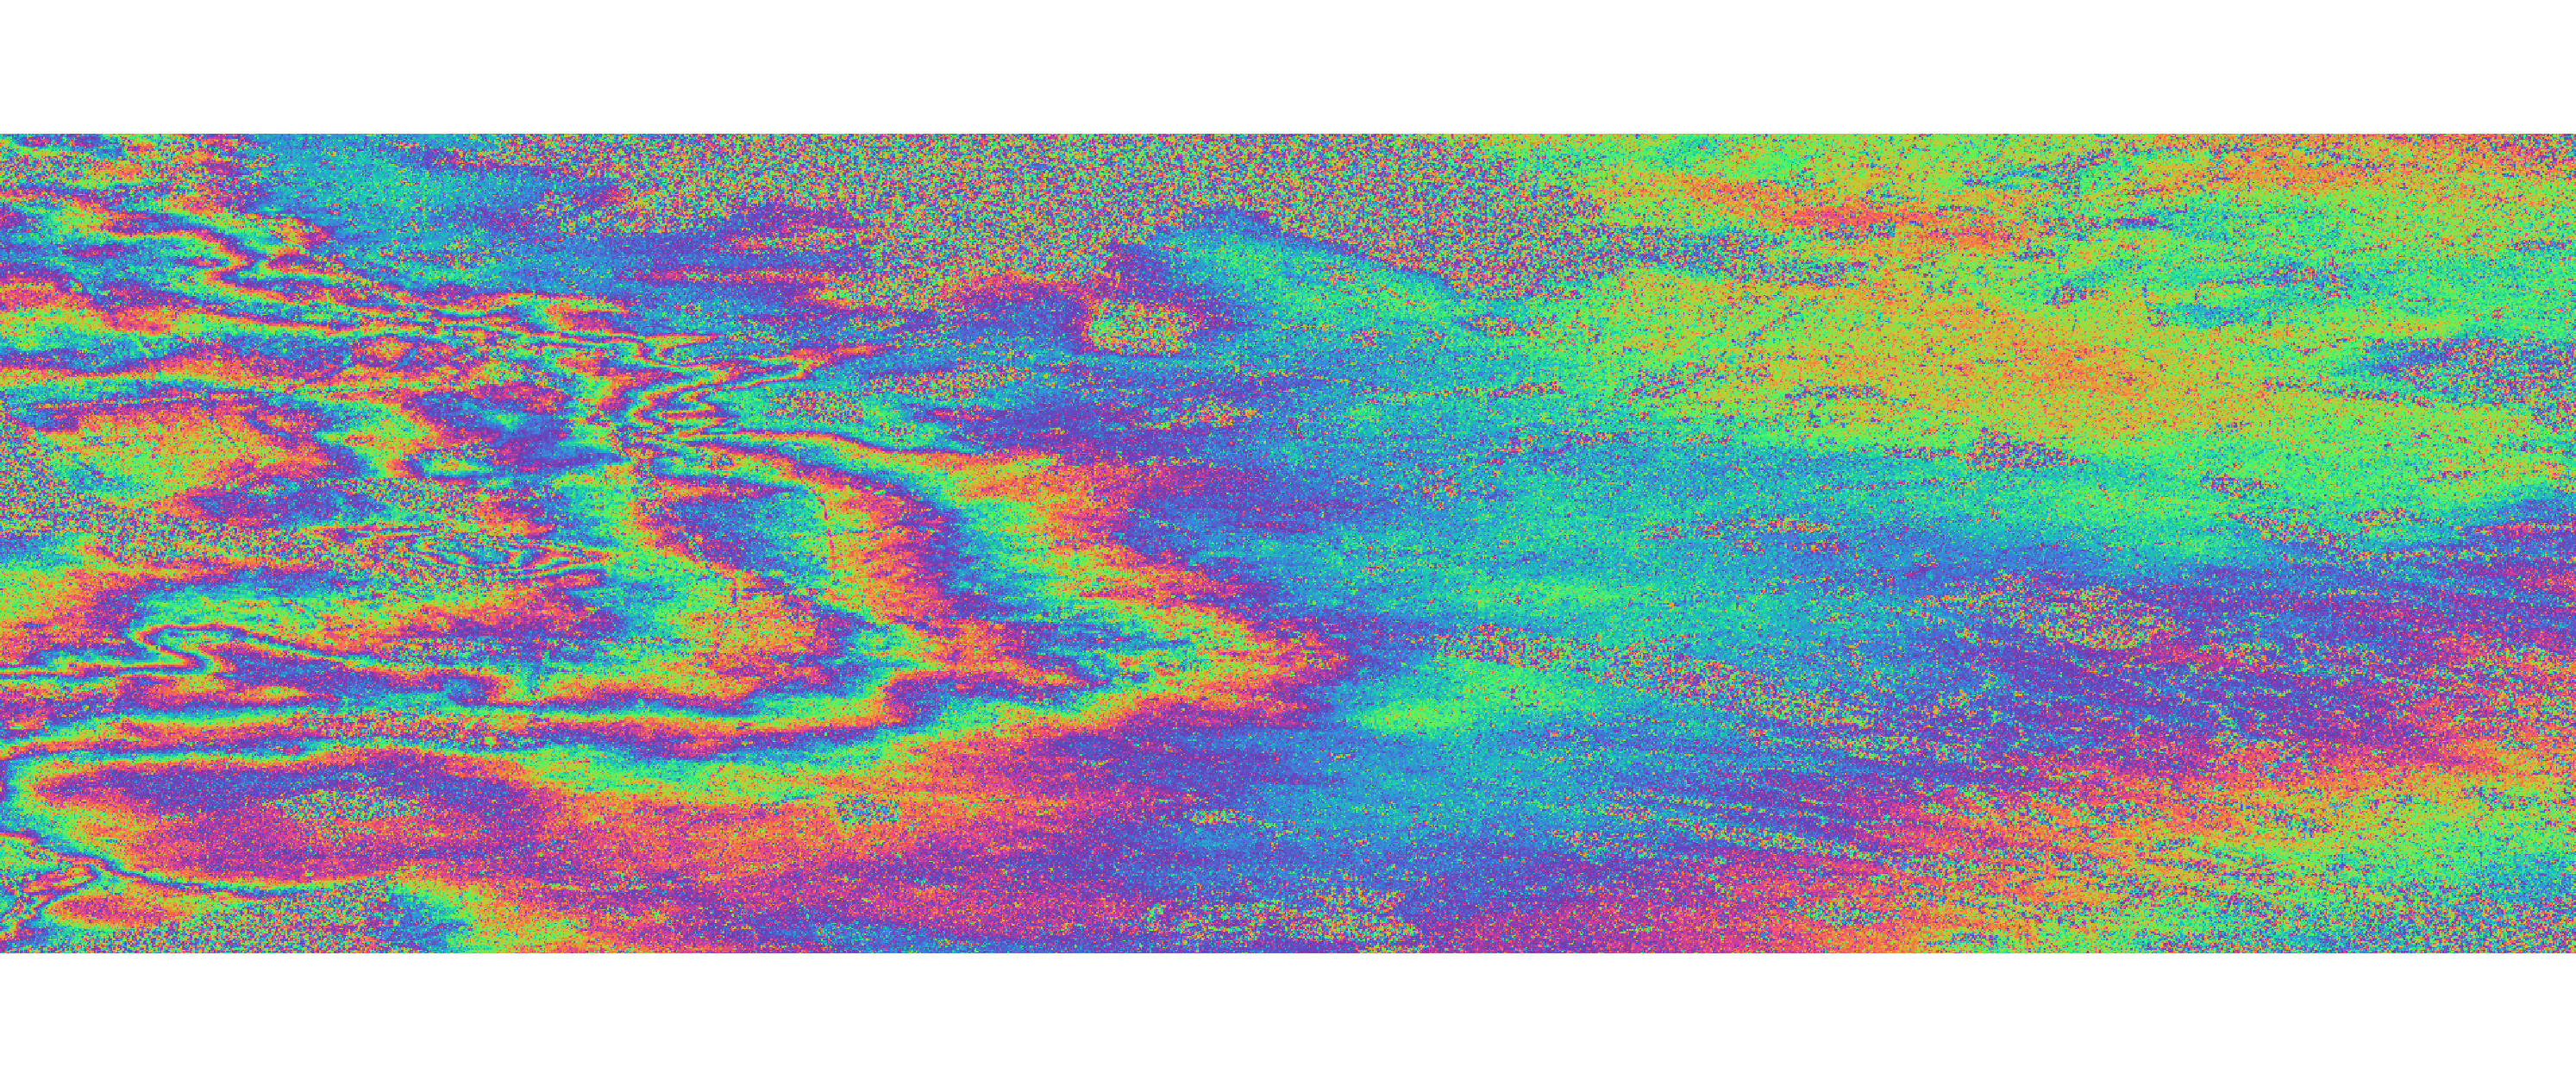
\includegraphics[trim={0 10cm 0 10cm},clip,width=0.8\textwidth]{images/real_data/offline_phase_SGPL_date_20_process=5_windowsize=8.png}
            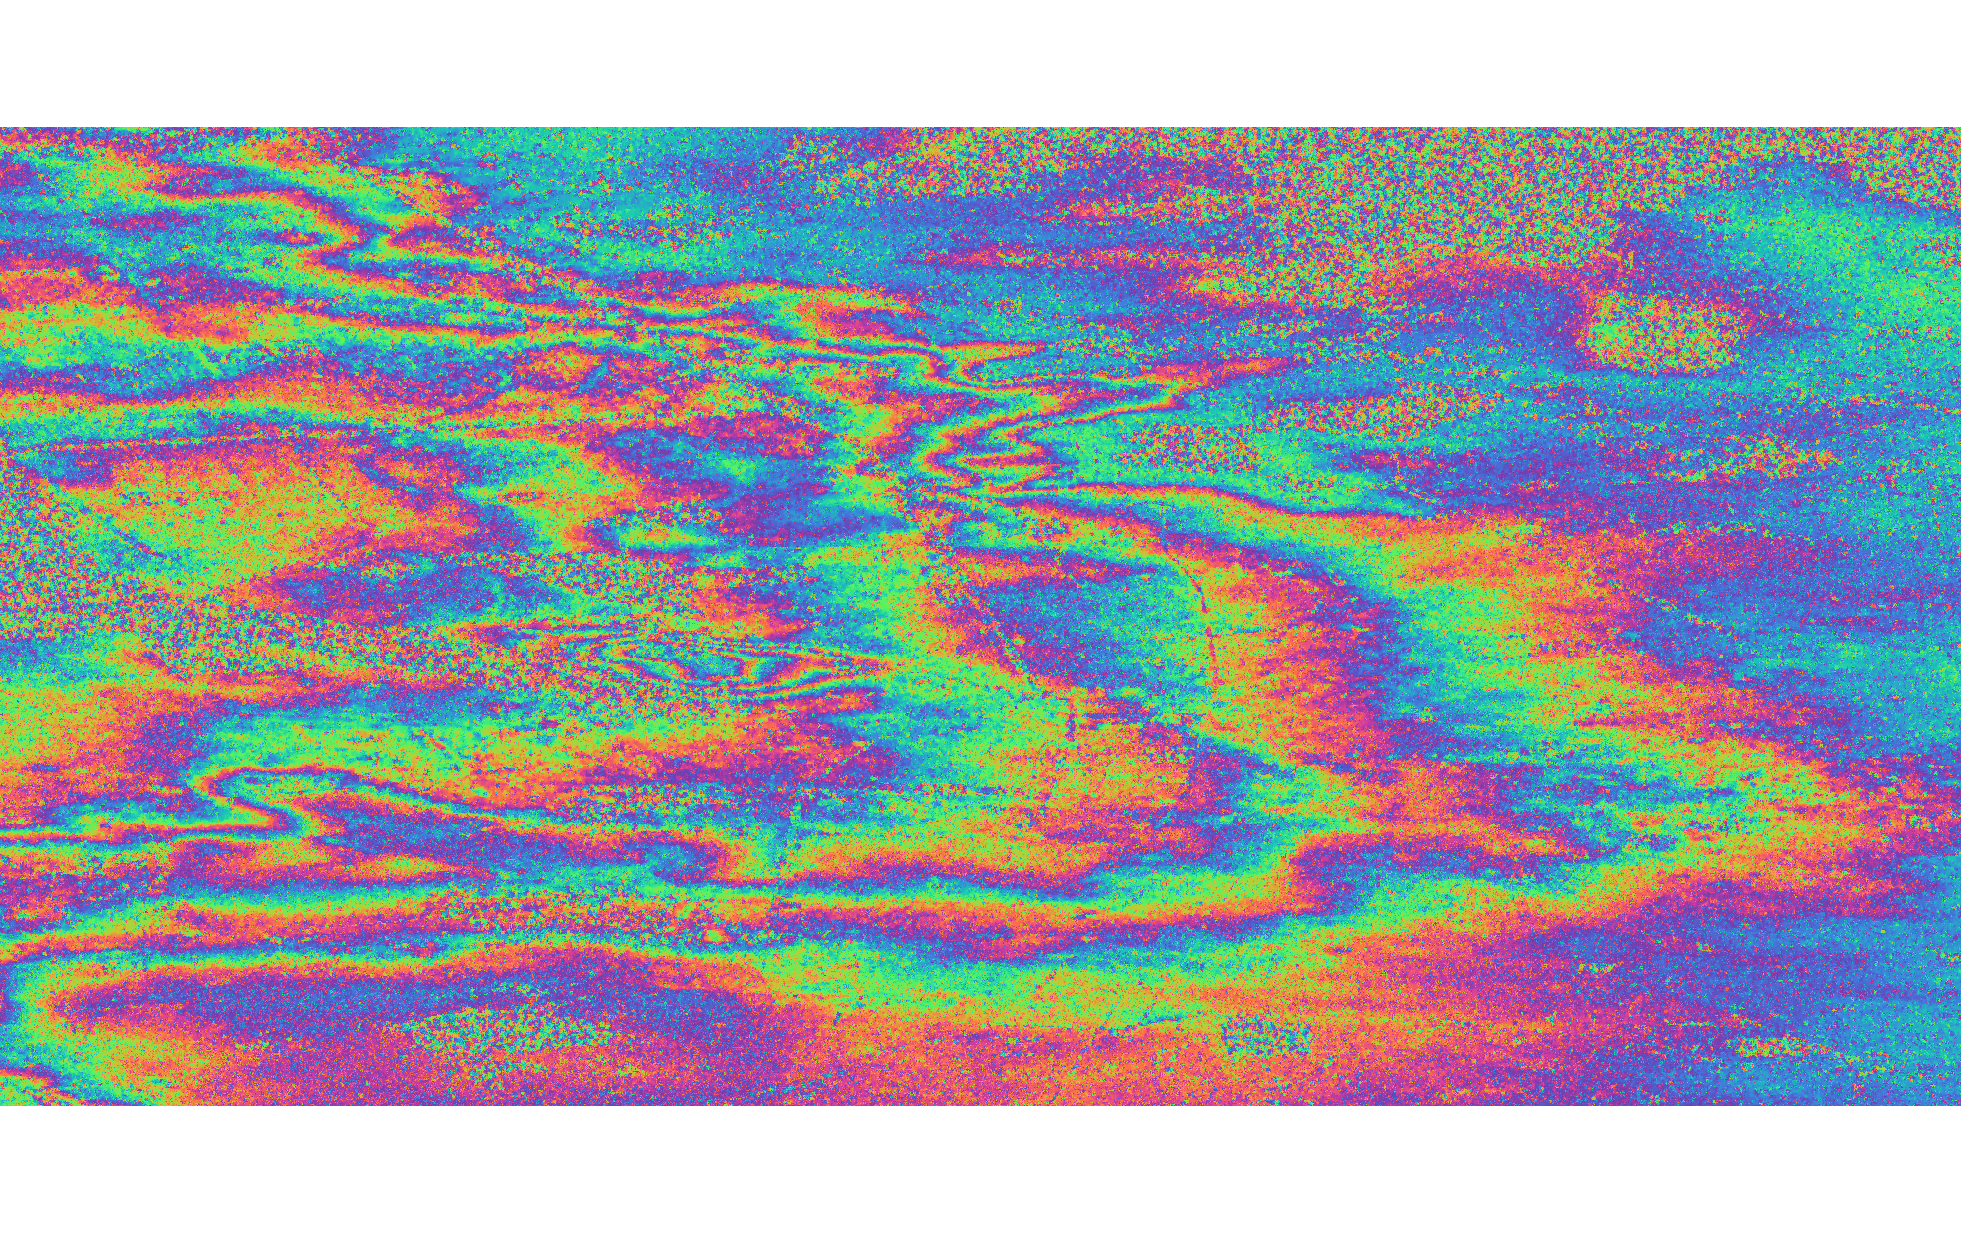
\includegraphics[width=0.6\textwidth]{images/real_data/SG_MLE_PL_l=20_phasecorrec_3_n_64_window_size=8_700_2700_6000_10000_date_20.png}
            \vspace{-1.5em}
            \caption{\footnotesize \acs{MLEPL}}
            \vspace{-1em}
        \end{subfigure}
        %\hfill
        \begin{subfigure}[b]{\columnwidth}
            \centering
            %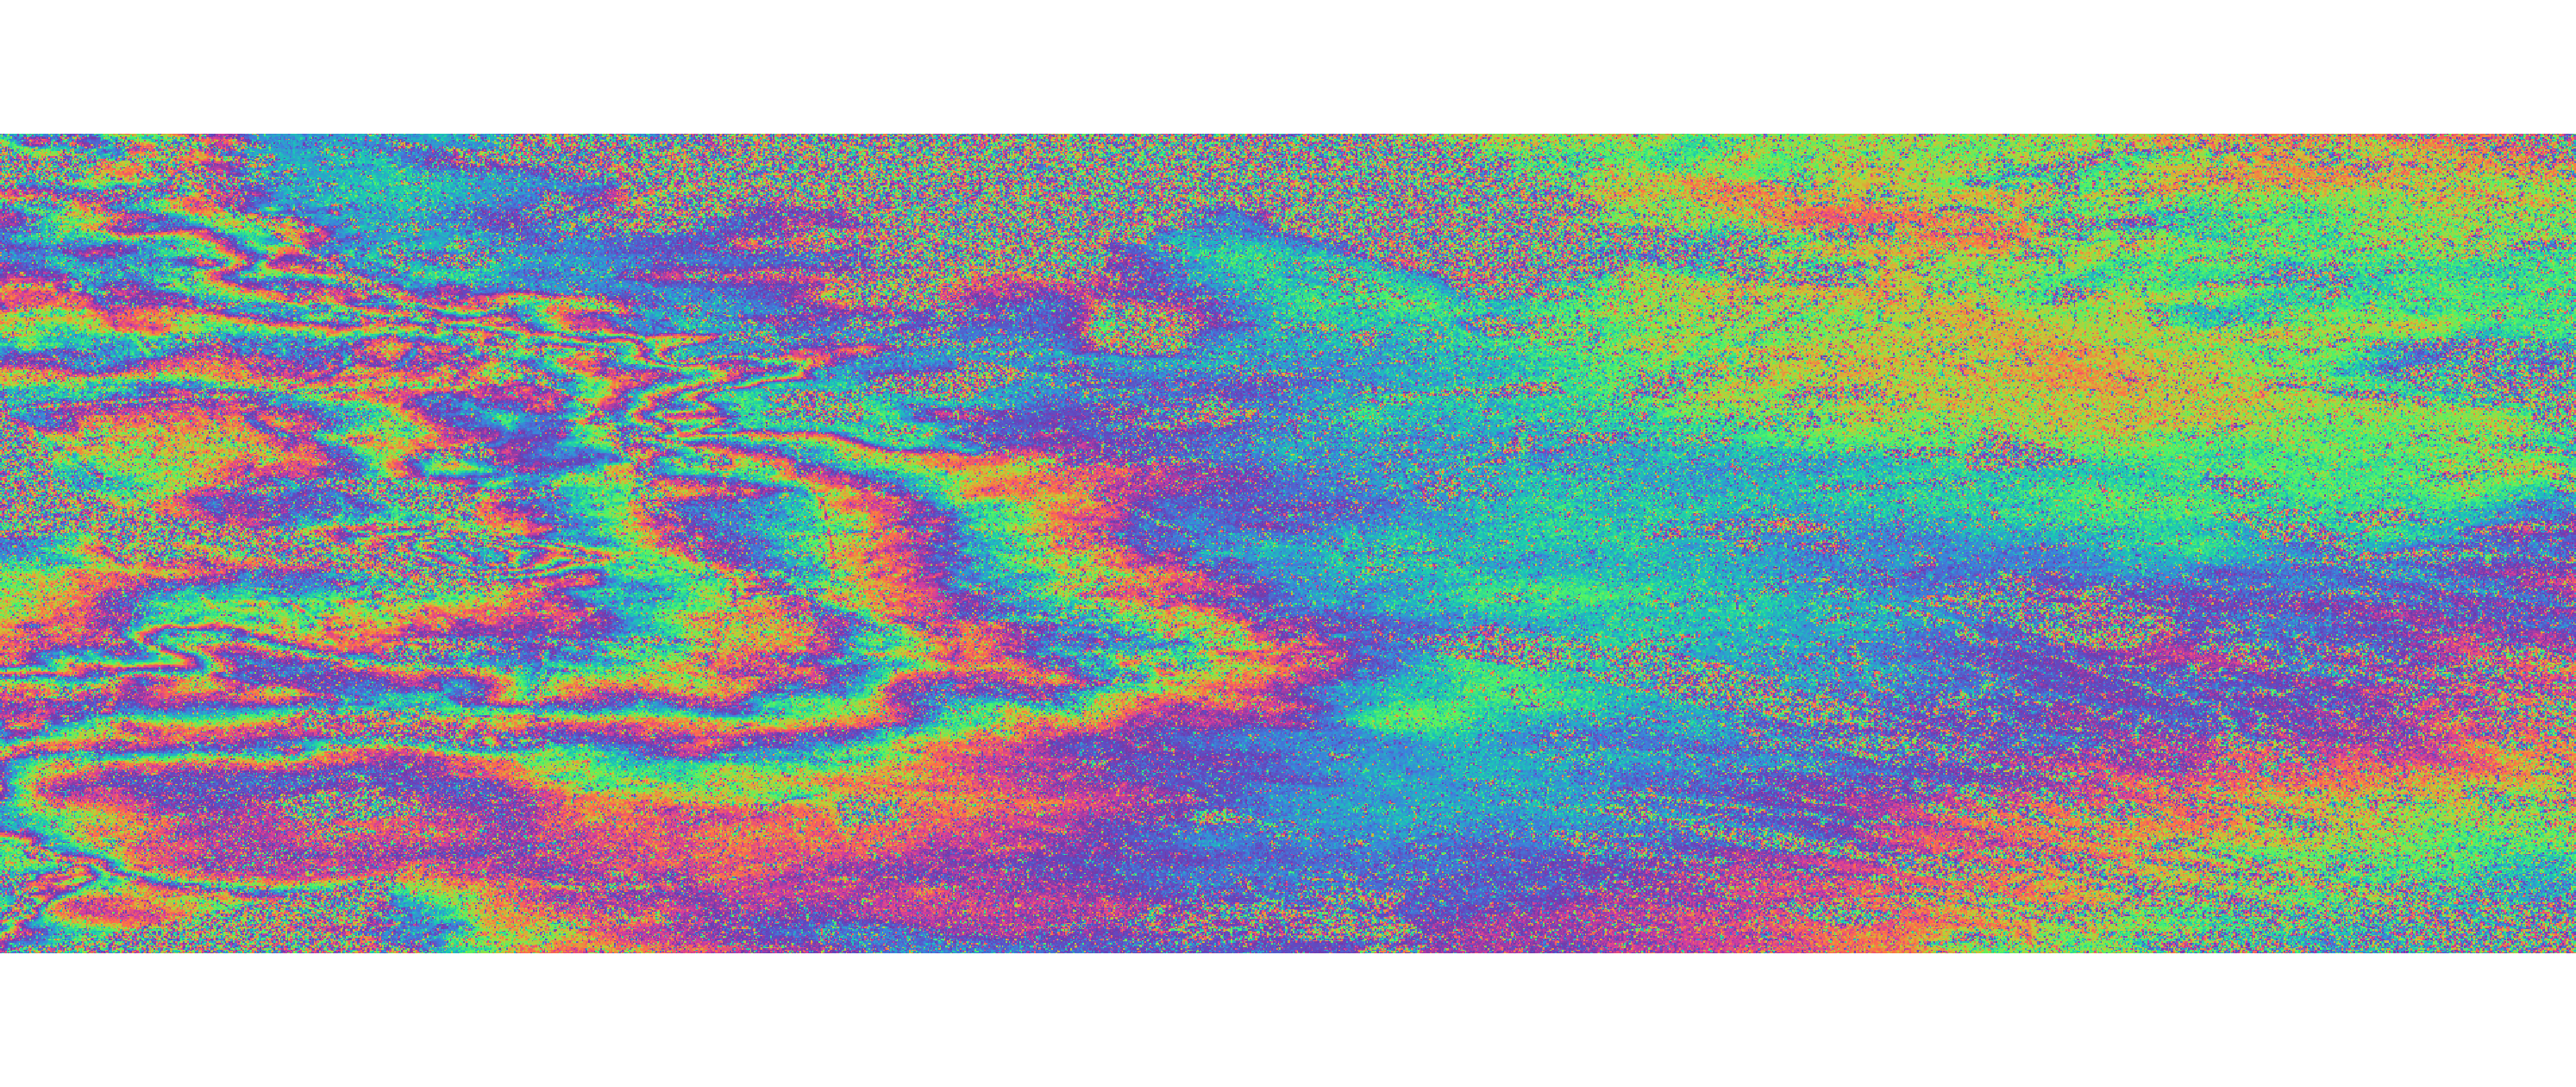
\includegraphics[trim={0 10cm 0 10cm},clip,width=0.8\textwidth]{images/real_data/phase_sequential_date_20_overlap=4_process=5.png}
            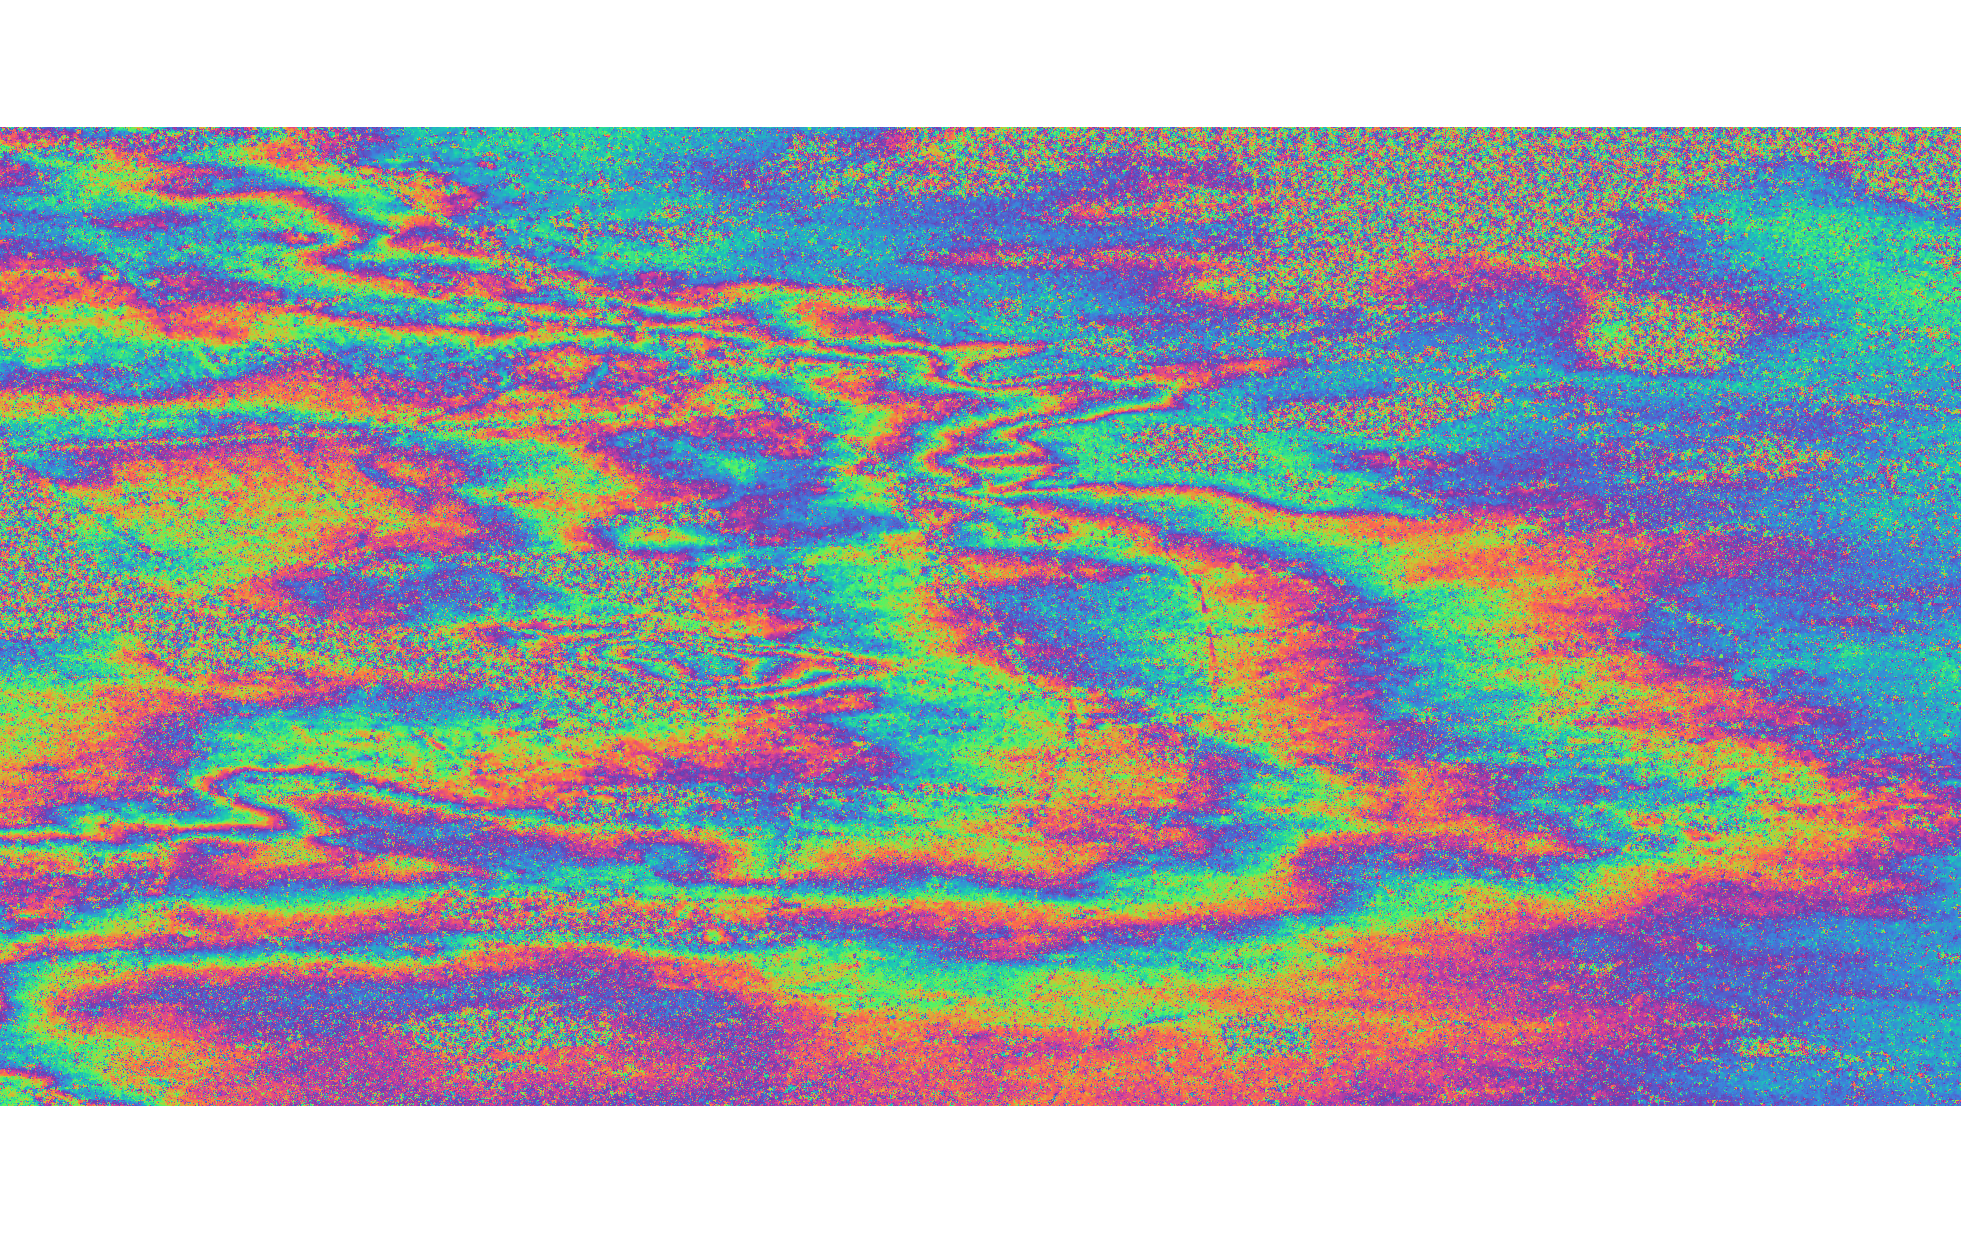
\includegraphics[width=0.6\textwidth]{images/real_data/S_SG_MLE_PL_l=20_phasecorrec_3_n_64_window_size=8_700_2700_6000_10000_date_20.png}
            \vspace{-1.5em}
            \caption{\footnotesize \acs{SMLEPL}}
            %\vspace{-1em}
        \end{subfigure}
        %\hfill
        \begin{subfigure}[b]{\columnwidth}
            \centering
            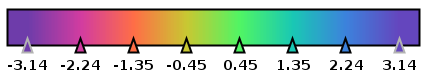
\includegraphics[width=0.5\textwidth, height=2.5em]{images/real_data/legend.png}
        \end{subfigure}
        \caption{\small Close-up view of the longest temporal baseline interferogram ($14$ August $2019$ - $10$ April $2020$) estimated by (a) \acs{MLEPL} \citep{vu2023robust} and (b) \acs{SMLEPL} in case $l = 20$ and $n = 64$.}
        \label{fig:real_data}
    \end{figure}
    \vspace{-0.7em}
    \noindent 
    Fig. \ref{fig:real_data} presents the longest temporal baseline interferogram %(phase differences) 
    estimated by \acs{MLEPL} \citep{vu2023robust}, \acs{SMLEPL}, with the multi-looking window, denoted as $n = 8 \times 8$, remains the same. The results are analyzed by comparing \acs{MLEPL} with our sequential approach. % estimation (our approach with \acs{sgMLEPL}), followed by a comparison within sequential estimation methods (our approach with the Sequential Estimator).
    Both approaches, \acs{MLEPL} and \acs{SMLEPL} yield the same results,  however the sequential approach demonstrates significantly faster execution time compared to the offline one when applied to real data. %\textcolor{blue}{
    Practically, the sequential approach took only $0.094$ hour, whereas the offline method required over $0.78$ hour using a machine with a $95$-core CPU running at $2.2$ GHz and $125$ G of RAM with calculations executed in parallel across the CPUs. Additionally, we compare the results of our approach with those of \citep{elhajjar2024} and  \citep{ansari2017sequential}. 
    %We compute the \acs{RMSE} between these sequential approaches and the offline result \acs{MLEPL} \citep{vu2023robust}, and we observe that our approach has a smaller value $\ac{MSE}_{\scriptsize \text{S-MLE-PL}} = 1.62$, while $\ac{MSE}_{\scriptsize \text{S-G-MLE-PL}} = 1.74$ and the Sequential Estimator \citep{ansari2017sequential} has a value $\ac{MSE}_{\scriptsize \text{Seq~Est}} = 1.89$. 
    Based on \citep{ansari2017sequential}, which used the \acl{RMSE} (\acs{RMSE}) criterion despite the ambiguity of the modulo $2 \pi$ in phase estimation, we compute the \acs{RMSE} between these sequential approaches and the offline result \ac{MLEPL} \citep{vu2023robust}. We observe that our approach yields a lower value of $\ac{RMSE}_{\scriptsize \text{S-MLE-PL}} = 1.62$, while $\ac{RMSE}_{\scriptsize \text{S-G-MLE-PL}} = 1.74$  and the Sequential Estimator \citep{ansari2017sequential} has an $\ac{RMSE}_{\scriptsize \text{Seq~Est}} = 1.89$.
    %}
    
    % machine ws1 ws2 : 
    % CPU : 96 core
    % CPU : 2.2 GHz
    % Mem : 128 Ram